\UseRawInputEncoding
\documentclass[10pt, letterpaper] {article}
\usepackage{natbib}
\usepackage{amsmath, amsthm, amssymb, mathrsfs,array}
\usepackage{graphicx,float,wrapfig,subfigure,color,pdfpages,fixltx2e,url}
\pagestyle{plain}
\setlength{\parskip} {11pt}
\setlength{\parindent} {2em}
\setlength{\textwidth}{6.5in}
\setlength{\oddsidemargin} {0in}
\setlength{\textheight} {8.5in}
\setlength{\topmargin} {-0.5in}
\parskip 7.2pt

\newcommand{\nnub}{\nonumber}
\newtheorem{theorem}{Theorem}
\newtheorem{lemma}{Lemma}
\newtheorem{transform}{Transformation}
\newtheorem{corollary}{Corollary}
\newtheorem{property}{Property}
%\newtheorem{proposition}{Proposition}[section]
\newtheorem{proposition}{Proposition}
\newtheorem{definition}{Definition}
\newtheorem{algorithm}{Algorithm}
\newtheorem{assumption}{Assumption}
\newtheorem{observation}{Observation}

\renewcommand{\baselinestretch}{1.5}

\newcommand{\vocab}[1]{\textcolor{red}{#1}}

\begin{document}
	\title{NUS Business School Honors Dissertation}
	\author{Peng Seng Ang}
	\date{AY 2019/2020 Semester 2}
	\maketitle
\begin{abstract}
This paper studies how we can use various spatial-temporal time series model to better predict demand across different locations. 
\end{abstract}
\section{Introduction}
Having an accurate forecast of delivery demand for food service providers would help them more effectively and efficiently assign orders to drivers to improve the overall delivery time. Currently, most Autoregressive (AR) or Autoregressive Integrated Moving Average (ARIMA) models only consider temporal features when predicting demand. However, we believe including spatial features between the data points might improve forecast accuracy. This paper would focus on and explore models that include both spatial and temporal features to improve forecast accuracy. 

\section{Literature Review}
To be written

\section{Data}
The data source used was an operational dataset from a food delivery service provider from Shanghai that includes delivery information for a 2-month period from 10 August 2015 to 30 September 2015 (excluding Saturdays) in 2015. The provider only provides delivery service for 90 minutes during lunchtime and the dataset has split the data into 15-minute time periods, and as such, each day would only consists of demand data for 6 time periods. Hence, our dataset has 839 locations with demand count data, in integer, for 204 time periods in total. 

To include other exogenous variables, data from https://www.worldweatheronline.com/shanghai-weather-history/shanghai/cn.aspx was used to include weather and rainfall data as well as encoding of the weekadys for all the respective days. 

\subsection{Exploratory Analysis}
We would first do some exploratory analysis and check if there are any obvious relationships between the variables.

\begin{figure}[H]
    \centering
    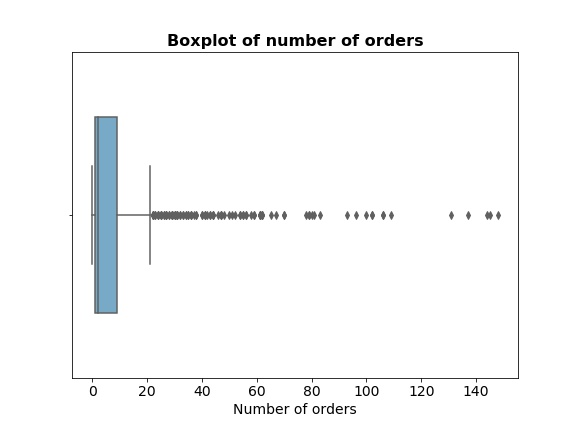
\includegraphics[width=\textwidth]{Images/boxplot_counts.jpg}
    \caption{Boxplot of counts}
    \label{fig:Boxplot of counts}
\end{figure}
We can see from the boxplot that most of the locations have extremely low number of non-zero orders, with about 335 locations having just a maximum of one non-zero order throughout the 204 time periods. 

\begin{figure}[H]
    \centering
    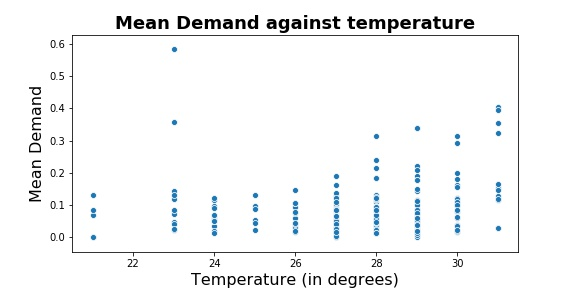
\includegraphics[width=\textwidth]{Images/temp_mean_demand.jpg}
    \caption{Scatter plot of mean counts against temperature}
    \label{fig:Scatter plot of mean counts against temperature}
\end{figure}

\begin{figure}[H]
    \centering
    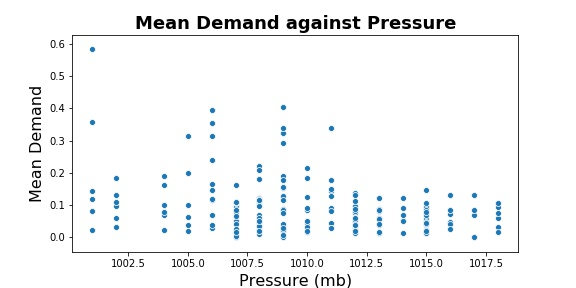
\includegraphics[width=\textwidth]{Images/pressure_mean_demand.jpg}
    \caption{Scatter plot of mean counts against pressure}
    \label{fig:Scatter plot of mean counts against pressure}
\end{figure}

The scatter plot in Figure 2 visually display a slight positive relationship between temperature and mean demand across all locations whereas Figure 3 visually display a slight negative relationship between pressure and mean demand across all locations. 

The distribution plots for the rest of the exogenous variables can be found in the appendix. 


\section{Baseline Model}
In this section, we would build a simple baseline model. Following which, we would try other different spatial temporal time series models and compare the results to the baseline model. 

\subsection{Metric Used}
The main metric that would be used for comparison would be Mean Squared Forecast Error (MSFE), which is calculated by:

\begin{center}
    %$\displaystyle MSFE=\frac{1}{(T_2 - T_1 - 1)}\sum_{t=T_1}^{T_2 - 1}\left \| \hat{y}_{t+1} - y_{t+1} \right \|_{2}^{2}$
    $\displaystyle MSFE=\frac{1}{n}\sum_{t=1}^{n}\left \| \hat{y}_{t} - y_{t} \right \|_{2}^{2}$
\end{center}
where \textit{n} is the number of data points, $\hat{y_t}$ is the predicted demand at time t and ${y_t}$ is the actual demand at time t.


\subsection{Train-Test Split}
From Figure 1 in Section 3.1, the data is very sparse as there are many locations that have no demand counts for the majority of the time period. Hence, to get a better idea of how our models would work, only locations with at least 50 non-zero counts across the time period would be used initially, leaving us with 42 locations that meet this criteria. The dataset was then split into training and test set by considering the first 27 days as the training set and the next 7 days as the test set. Our training set would then have 162 demand data for each location and test set would have 42 demand data for each location. 

\subsection{ARIMA models}
Autoregressive Integrated Moving Average (ARIMA) models are one of the most commonly used models for time series (\cite{Asha2016}). ARIMA models are made up of 3 processes, mainly the Autoregressive (AR) process, the Integrated (I) process and the Moving Average (MA) process (\cite{Jamal2018}). The AR process assumes that each observation can be expressed as a linear combination of its past values.  An AR(x) process would mean using x lagged values. The MA process assumes that each observation can be expressed as a linear combination of its current error term as well as its past error terms. The Integrated Process states that the time series can undergo differencing to ensure that the series is stationary. A MA(x) process would mean using x number of past observations. Hence, an ARIMA model is usually represented by ARIMA(p,d,q), where \textit{p} represents the number of autoregressive terms, \textit{d} represents the number of differences needed for stationarity, and \textit{q} represents the number of lagged forecast errors. 

\subsection{Baseline ARIMA Result}
As a baseline model, each of the locations was assessed individually and a suitable ARIMA model was built for each location. Auto-arima function from Python was used to implement this. The out-of-sample MSFE for this baseline model on the 42 locations is \textbf{58.80}. A sample forecast plot is shown below:

\begin{figure}[H]
    \centering
    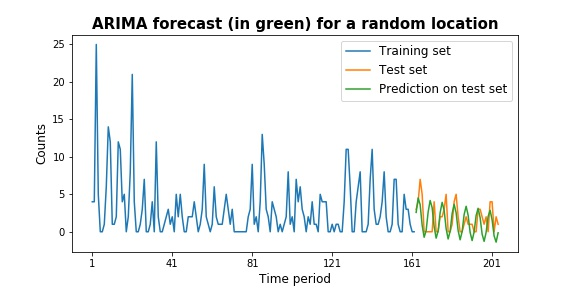
\includegraphics[width=\textwidth]{Images/forecast_example.jpg}
    \caption{ARIMA forecast on a random location}
    \label{fig:ARIMA forecast on a random location}
\end{figure}



\section{VAR Model}
Vector Autoregressive (VAR) models are the most commonly used model for multivariate time series, particularly in economics and financial time series as shown in \cite{Hilde2000}. VAR models are very similar to multivariate linear regression models and methods used to perform inferencing on linear regression models can also be applied to VAR models. VAR(p) represents a VAR model of order p if the time series can be written as: 

\begin{center}
    $\displaystyle y_t=v+\sum_{i=1}^{p} \phi_{i}y_{t-i}+\alpha_t$
\end{center}

\noindent where $p$ is the number of lagged endogenous variables used, $y_t$ is the value at time $t$, $v$ is a constant vector, $\phi_i$ are coefficient matrices for $i>0$ and $\alpha_t$ are independent and identically distributed random vectors. 

\subsection{Stationarity Condition}
For a univariate time series, it is important for the time series to be transformed into a stationary series and Augmented Dickey-Fuller (ADF) test can be used to perform unit root test for stationarity, as shown in \cite{Zhijie1998} and \cite{Rizwan2011}. For a multi-variate time series, if the series are unit-root non-stationary, applying the VAR model could lead to spurious regression, as shown in \cite{Baumohl2009}. While it is possible to perform differencing on every series, it might cause over-differencing, as mentioned in \cite{Ruey2014}. In this paper, we would check for cointegration between the series instead. 

\subsubsection{Cointegration}
\cite{Box1977} shows that it is possible to linearly combine various unit-root nonstationary time series to form a stationary series. The term Cointegration, first mentioned in \cite{Granger1983}, states that although some or all the time series might be unit-root nonstationary individually, these time series can be said to be cointegrated if there exists a possible linear combination of them that would form a stationary series. Intuitively, 2 series are cointegrated if they move together and the distance between them remain stable over time. 

\subsubsection{Johansen Test for Cointegration}
While Cointegrated Augmented Dickey Fuller Test, commonly used for Pairs Trading, can be used, it is only able to be applied on 2 separate series. In our dataset, we have 839 locations at least, hence we would apply the popular approach to cointegrating tests for VAR model, called the Johansen's Cointegration Test. However, one limitation is that it can only be used to check for cointegration between a maximum of 12 variables. For further elaboration on the Johansen's Cointegration Test, please refer to \cite{Johansen1991}. 

\subsection{VARX Model}
VAR models can also be extended to include exogenous variables. A VARX(p,s) (with exogenous variables) model can be expressed as:

\begin{center}
    $\displaystyle y_t=v+\sum_{i=1}^{p} \phi_{i}y_{t-i}+\sum_{j=1}^{s} \beta_{j}x_{t-j}+\alpha_t$
\end{center}

\noindent where $p$ is the number of lagged endogenous variables used, $s$ is the number of lagged exogenous variables used, $y_t$ is the value at time $t$, $v$ is a constant vector, $\phi_i$ are coefficient matrices for endogenous coefficient matrix for $i>0$, $\beta_i$ are coefficient matrices for exogenous coefficient matrix for $i>0$ and $\alpha_t$ are independent and identically distributed random vectors. 

\subsection{Model Checking}
To validate and verify if our fitted model is adequate, model checking would be performed by performing the following residual analysis:

\subsubsection{Whiteness of Residuals}
To ensure our fitted model is adequate, the resiudals should behave like a white noise series. 

\subsubsection{Correlation of Residuals}


\subsection{Results}
BigVAR library in R was used to implement the VAR models. The results from the VAR model without exogenous variables gives an out-of-sample MSFE of XXX on the 42 locations. 


\section{GLM Model}
Since the dataset that we are using follows a count time series, it is worth exploring another class of model that is commonly used for this, which is the Generalized Linear Model (GLM). 

\subsection{Model Checking}
To validate our model,

\subsection{Insights and Implementation}
Any findings from the results? If there are any benefits or issues in implementing the proposed model...

\section{Limitations}

\section{Conclusion}
Conclude your efforts and main findings.

\section{Appendix}
Append extra plots, graphs, analysis, etc. 

%%%%%%%%%%%%%%%%%%%%%%%%%%%%%%%%%%%%%%%%%%%%%%%%%%%%%%%%%%%%
%%% Bibliography
%%%%%%%%%%%%%%%%%%%%%%%%%%%%%%%%%%%%%%%%%%%%%%%%%%%%%%%%%%%%
\bibliographystyle{apa} 
\bibliography{references}

\end{document}
